\chapter{Datenbank}
\newcounter{ids}

    \begin{figure}[h]
        \centering
        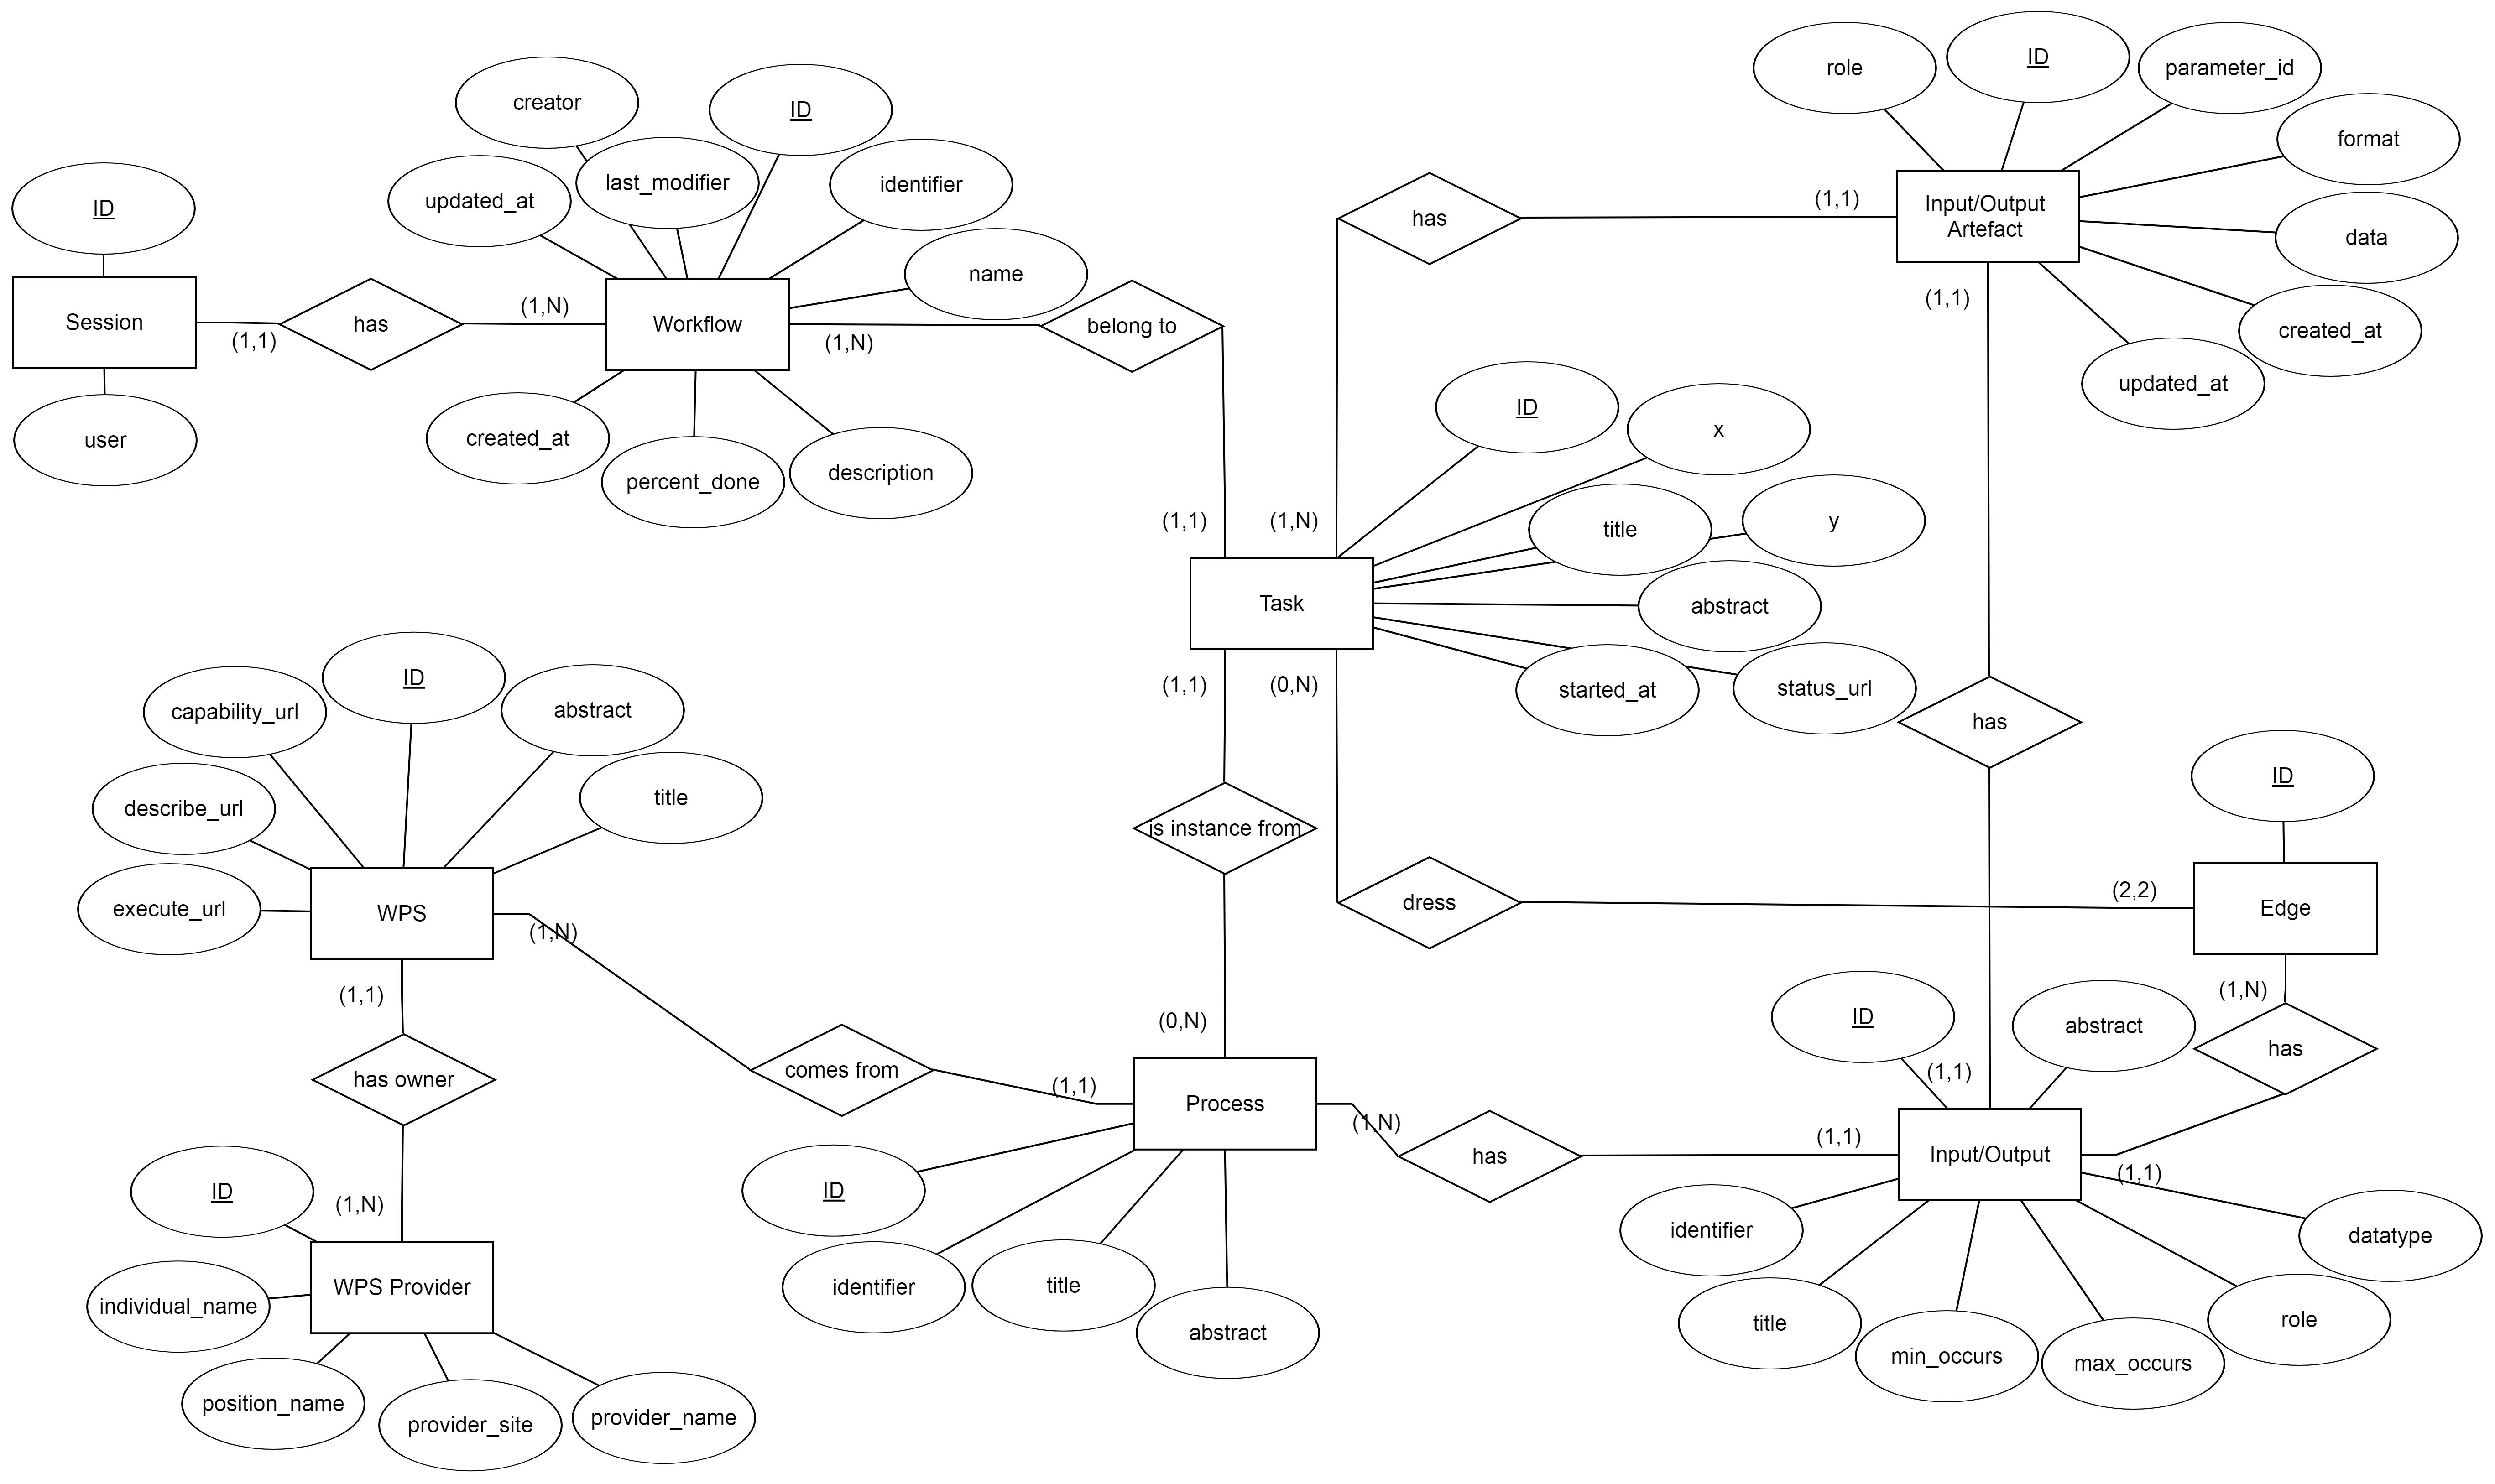
\includegraphics[width=15cm]{diagrams/ERDiagramm.png}
        \caption{Entity Relationship Diagram}
        \label{fig:er_diagramm}
    \end{figure}
    
    
	\section{Einleitung}
	
	hier kann sich jemand einen schönen text für ausdenken...
	
	
	\section{Tabellen}
	
% 		\subsection{ExecutionStatus}
% 		\begin{center}
% 			\setlength\tabcolsep{5pt}
% 			\renewcommand{\arraystretch}{1.5}
% 			\setcounter{ids}{0}			
% 			\begin{tabular}{|c|c|}
% 				\hline
% 				\rowcolor[gray]{0.75}[4.85pt]
% 				id & status\_value \\ \hline 
% 				\stepcounter{ids}\arabic{ids} & READY \\ \hline
% 				\stepcounter{ids}\arabic{ids} & WAITING \\ \hline
% 				\stepcounter{ids}\arabic{ids} & RUNNING \\ \hline
% 				\stepcounter{ids}\arabic{ids} & FINISHED \\ \hline
% 				\stepcounter{ids}\arabic{ids} & FAILED \\ 
% 				\hline
% 			\end{tabular}
% 		\end{center}
	      
    
	   % \subsection{DataType}
	   % \begin{center}
	   % 	\setlength\tabcolsep{5pt}
	   % 	\renewcommand{\arraystretch}{1.5}
	   % 	\setcounter{ids}{0}			
	   % 	\begin{tabular}{|c|c|}
	   % 		\hline
	   % 		\rowcolor[gray]{0.75}[4.85pt]
	   % 		id & type\_value \\ \hline 
	   % 		\stepcounter{ids}\arabic{ids} & LiteralData \\ \hline
	   % 		\stepcounter{ids}\arabic{ids} & ComplexData \\ \hline
	   % 		\stepcounter{ids}\arabic{ids} & BoundingBoxData \\ 
	   % 		\hline
	   % 	\end{tabular}
	   % \end{center}
	
	
% 		\subsection{ProcessHandler}
% 		\begin{center}
% 			\setlength\tabcolsep{5pt}
% 			\renewcommand{\arraystretch}{1.5}
% 			\setcounter{ids}{0}			
% 			\begin{tabular}{|c|c|}
% 				\hline
% 				\rowcolor[gray]{0.75}[4.85pt]
% 				id & handler\_name \\ \hline 
% 				\stepcounter{ids}\arabic{ids} & sayhello \\ \hline
% 				\stepcounter{ids}\arabic{ids} & wait \\ \hline
% 				\stepcounter{ids}\arabic{ids} &  \\ 
% 				\hline
% 			\end{tabular}
% 		\end{center}
		
		
		
% 		\subsection{Session}
% 		\begin{center}
% 			\setlength\tabcolsep{5pt}
% 			\renewcommand{\arraystretch}{1.5}
% 			\setcounter{ids}{0}			
% 			\begin{tabular}{|c|c|c|}
% 				\hline
% 				\rowcolor[gray]{0.75}[4.85pt]
% 				id & user\_id & last\_workflow\_id \\ \hline  
% 				\stepcounter{ids}\arabic{ids} & 1 & 1 \\ \hline
% 				\stepcounter{ids}\arabic{ids} & 1 & 1 \\	
% 				\hline
% 			\end{tabular}
% 		\end{center}		


% 		\subsection{ServiceProvider}
% 		\begin{center}
% 			\setlength\tabcolsep{5pt}
% 			\renewcommand{\arraystretch}{1.5}
% 			\setcounter{ids}{0}			
% 			\begin{tabular}{|c|c|c|}
% 				\hline
% 				\rowcolor[gray]{0.75}[4.85pt]
% 				id & provider\_name & provider\_site \\ \hline  
% 				\stepcounter{ids}\arabic{ids} & Test1 & test.useful.com \\ \hline
% 				\stepcounter{ids}\arabic{ids} & Test2 & test.nonsense.com \\	
% 				\hline
% 			\end{tabular}
% 		\end{center}		

		\subsection{Edge}
		\begin{center}
			\setlength\tabcolsep{5pt}
			\renewcommand{\arraystretch}{1.5}
			\setcounter{ids}{0}			
			\begin{tabular}{|c|c|c|}
				\hline
				\rowcolor[gray]{0.75}[4.85pt]
				id & workflow & from\_task & provider\_site \\ \hline  
				\stepcounter{ids}\arabic{ids} & Test1 & test.useful.com \\ \hline
				\stepcounter{ids}\arabic{ids} & Test2 & test.nonsense.com \\	
				\hline
			\end{tabular}
		\end{center}		
		

	
		
		\newpage
		
		\paperwidth=\pdfpageheight
		\paperheight=\pdfpagewidth
		\pdfpageheight=\paperheight
		\pdfpagewidth=\paperwidth
		\headwidth=1.05\textheight
		
		\begingroup 
		\vsize=\textwidth
		\hsize=1.05\textheight
		
		\textwidth=\hsize
		\textheight=\vsize


% 		\subsection{Service}
% 		\begin{center}
% 			\setlength\tabcolsep{5pt}
% 			\renewcommand{\arraystretch}{1.5}
% 			\setcounter{ids}{0}			
% 			\begin{tabularx}{\textwidth}{|l|l|l|l|l|l|X|}
% 				\hline
% 				\rowcolor[gray]{0.75}[4.85pt]
% 				id & service\_provider & capabilities\_url & describe\_url & execute\_url & service\_title & service\_abstract \\ \hline  
% 				\stepcounter{ids}\arabic{ids} & 1 & 1 & & & & \\ \hline
% 				\stepcounter{ids}\arabic{ids} & 1 & 1 & & & & \\	
% 				\hline
% 			\end{tabularx}
% 		\end{center}	
		
%		
%		\subsection{User}   
%		\begin{center}
%			\setlength\tabcolsep{5pt}
%			\renewcommand{\arraystretch}{1.5}
%			\setcounter{ids}{0}			
%			\begin{tabularx}{\textwidth}{|l|l|l|l|l|l|X|}
%				\hline
%				\rowcolor[gray]{0.75}[4.85pt]
%				id & user\_login & user\_pw & user\_name & user\_prename & user\_mail & user\_level \\ \hline
%				\stepcounter{ids}\arabic{ids} & admin & \$P\$D5pZ02d5vO/g9FAmkbZQIKaT3cW6zW1 & Min & Ad & admin@pseworkflow.scc.kit.edu & admin \\ \hline 
%				\stepcounter{ids}\arabic{ids} & & & & & & \\
%				\hline
%			\end{tabularx}
%		\end{center}
			
			
		\subsection{Task}
		\begin{center}
			\setlength\tabcolsep{5pt}
			\renewcommand{\arraystretch}{1.5}
			\setcounter{ids}{0}			
			\begin{tabularx}{\textwidth}{|l|l|l|l|l|l|l|l|l|X|}
				\hline
				\rowcolor[gray]{0.75}[4.85pt]
				id & workflow & process & x & y & status & title & status\_url & started\_at & abstract \\ \hline  
				&&&&&&&&& \\
				\hline
			\end{tabularx}
		\end{center} 
		
		
		\subsection{Workflow}
		\begin{center}
			\setlength\tabcolsep{5pt}
			\renewcommand{\arraystretch}{1.5}
			\setcounter{ids}{0}			
			\begin{tabularx}{\textwidth}{|l|l|l|l|l|l|l|l|l|X|}
				\hline
				\rowcolor[gray]{0.75}[4.85pt]
				id & wf\_identifier & wf\_title & wf\_abstract & wf\_status & wf\_owner & wf\_shared\_with & wf\_num\_tasks & wf\_percent\_done & wf\_exectuable \\ \hline 
				\stepcounter{ids}\arabic{ids} & test\_wf & Test WF & Nur zum Test & RUNNING & admin &  & 2 & 50 & true \\ \hline
				\stepcounter{ids}\arabic{ids} & & & & & & & & & \\ 
				\hline
			\end{tabularx}
		\end{center}
		
		
		
		\subsection{Data}
		\begin{center}
			\setlength\tabcolsep{5pt}
			\renewcommand{\arraystretch}{1.5}
			\setcounter{ids}{0}			
			\begin{tabularx}{\textwidth}{|l|l|l|l|l|l|l|l|l|X|}
				\hline
				\rowcolor[gray]{0.75}[4.85pt]
				id & task\_id & data\_IO & data\_identifier & data\_title & data\_abstract & data\_type & data\_min\_occurs & data\_max\_occurs & data\_value \\ \hline 
				\stepcounter{ids}\arabic{ids} & 1 & input & & & & LiteralData & 1 & 1 & Admin \\ \hline
				\stepcounter{ids}\arabic{ids} & 2 & input & & & wait 20 ms & LiteralData & 1 & 1 & 20 \\ \hline
				\stepcounter{ids}\arabic{ids} & 1 & output & & & & LiteralData & 1 & 1 & "Hello Admin" \\ \hline
				\stepcounter{ids}\arabic{ids} & & & & & & & & & \\ 
				\hline
			\end{tabularx}
		\end{center}
		
		

		
		
		
	\endgroup
	\newpage
	\paperwidth=\pdfpageheight
	\paperheight=\pdfpagewidth
	\pdfpageheight=\paperheight
	\pdfpagewidth=\paperwidth
	\headwidth=\textwidth
	
        
    \section{Kommunikationsmodell}
	    
	    hier schemazeichnung von den komponenten (servern, etc) und pfeile mit kommunikationsrichtung, um datenverkehr darzustellen. daraus soll hervorgehen, dass datenbank das datenkonsistenzglied ist
	    